\subsection{Carrera a la que pertenecen los estudiantes:}

A continuación se muestra un cuadro con los datos de cualitativos de las carreras de los estudiantes pertenecientes a muestra, se pretender hacer una ordenación de los mismos, generar una tabla de frecuencias y establecer una gráfica representativa.

\begin{table}[H]
  \centering
  \hspace*{-2cm} % Mueve la primera tabla más a la izquierda
  \begin{minipage}{0.35\textwidth} % Ajustar el ancho según sea necesario
    \centering
    \begin{tabular}{l @{\hskip 0.6cm} l}
      \hline
      \textbf{Carrera} & \textbf{Acrónimo} \\ \hline
      Ingeniería       & \small{ING}                \\ \hline
      Psicología       & \small{PSI}                \\ \hline
      Comunicaciones   & \small{COM}                \\ \hline
      Arquitectura     & \small{ARQ}                \\ \hline
      Derecho          & \small{DER}                \\ \hline
      Administración   & \small{ADM}                \\ \hline
      Negocios         & \small{NEG}                \\ \hline
      Medicina         & \small{MED}                \\ \hline
      Gastronomía      & \small{GAS}               \\ \hline
    \end{tabular}
    \caption{Carreras y acrónimos de los estudiantes en la muestra.}
    \label{tab:carreras-acronimos}
  \end{minipage}
  \hspace{0.2cm} % Espacio horizontal entre las tablas
  \begin{minipage}{0.45\textwidth} % Ajustar el ancho según sea necesario
    \centering
    \caption{Representación de Carreras}
    \begin{tabular}{|>{\scriptsize}m{0.6cm}|>{\scriptsize}m{0.6cm}|>{\scriptsize}m{0.6cm}|>{\scriptsize}m{0.6cm}|>{\scriptsize}m{0.6cm}|>{\scriptsize}m{0.6cm}|>{\scriptsize}m{0.6cm}|>{\scriptsize}m{0.6cm}|>{\scriptsize}m{0.6cm}|>{\scriptsize}m{0.6cm}|} \hline \scriptsize{\textbf{ING}} & \scriptsize{\textbf{ING}} & \scriptsize{\textbf{ING}} & \scriptsize{\textbf{ING}} & \scriptsize{\textbf{ING}} & \scriptsize{\textbf{ING}} & \scriptsize{\textbf{ING}} & \scriptsize{\textbf{ING}} & \scriptsize{\textbf{ING}} & \scriptsize{\textbf{ING}} \\ \hline \scriptsize{\textbf{ING}} & \scriptsize{\textbf{ING}} & \scriptsize{\textbf{ING}} & \scriptsize{\textbf{ING}} & \scriptsize{\textbf{ING}} & \scriptsize{\textbf{ING}} & \scriptsize{\textbf{ING}} & \scriptsize{\textbf{ING}} & \scriptsize{\textbf{ING}} & \scriptsize{\textbf{ING}} \\ \hline \scriptsize{\textbf{ING}} & \scriptsize{\textbf{ING}} & \scriptsize{\textbf{ING}} & \scriptsize{\textbf{ING}} & \scriptsize{\textbf{ING}} & \scriptsize{\textbf{ING}} & \scriptsize{\textbf{ING}} & \scriptsize{\textbf{ING}} & \scriptsize{\textbf{ING}} & \scriptsize{\textbf{ING}} \\ \hline \scriptsize{\textbf{ING}} & \scriptsize{\textbf{ING}} & \scriptsize{\textbf{ING}} & \scriptsize{\textbf{ING}} & \scriptsize{\textbf{ING}} & \scriptsize{\textbf{ING}} & \scriptsize{\textbf{ING}} & \scriptsize{\textbf{ING}} & \scriptsize{\textbf{ING}} & \scriptsize{\textbf{ING}} \\ \hline \scriptsize{\textbf{ING}} & \scriptsize{\textbf{ING}} & \scriptsize{\textbf{ING}} & \scriptsize{\textbf{ING}} & \scriptsize{\textbf{ING}} & \scriptsize{\textbf{DER}} & \scriptsize{\textbf{DER}} & \scriptsize{\textbf{DER}} & \scriptsize{\textbf{PSI}} & \scriptsize{\textbf{PSI}} \\ \hline \scriptsize{\textbf{PSI}} & \scriptsize{\textbf{PSI}} & \scriptsize{\textbf{PSI}} & \scriptsize{\textbf{MED}} & \scriptsize{\textbf{COM}} & \scriptsize{\textbf{ARQ}} & \scriptsize{\textbf{ARQ}} & \scriptsize{\textbf{ADM}} & \scriptsize{\textbf{ADM}} & \scriptsize{\textbf{ADM}} \\ \hline \scriptsize{\textbf{ADM}} & \scriptsize{\textbf{NEG}} & \scriptsize{\textbf{NEG}} & \scriptsize{\textbf{NEG}} & \scriptsize{\textbf{NEG}} & \scriptsize{\textbf{NEG}} & \scriptsize{\textbf{GAS}} & & & \\ \hline \end{tabular}
  \end{minipage}
\end{table}

\textbf{Tabla de frecuencias:}

El siguiente cuadro muestra la distribución de carreras de los participantes en la muestra, dividiéndose en las diferentes opciones de carrera, así mismo se muestra la frecuencia absoluta, acumulada, relativa porcentual y relativa porcentual acumulada.

% Tenemos estos datos:

% Ing: 55
% Der: 3
% Psi: 5
% Med: 1
% Com: 1
% Arq: 2
% Adm: 4
% Neg: 5
% Gast: 1

\begin{table}[H]
  \centering
  \begin{tabular}{l @{\hskip 0.6cm} c @{\hskip 0.6cm} c @{\hskip 0.6cm} c @{\hskip 0.6cm} c}
    \hline
    \textbf{Carrera} & \textbf{$f_i$} & \textbf{$F_i$} & \textbf{$h_i$ (\%)} & \textbf{$H_i$ (\%)} \\ \hline
    Ingeniería       & 55             & 55             & 71.43               & 71.43               \\ \hline
    Derecho          & 3              & 58             & 3.90                & 75.32               \\ \hline
    Psicología       & 5              & 63             & 6.49                & 81.82               \\ \hline
    Medicina         & 1              & 64             & 1.30                & 83.12               \\ \hline
    Comunicaciones   & 1              & 65             & 1.30                & 84.42               \\ \hline
    Arquitectura     & 2              & 67             & 2.60                & 87.01               \\ \hline
    Administración   & 4              & 71             & 5.19                & 92.21               \\ \hline
    Negocios         & 5              & 76             & 6.49                & 98.70               \\ \hline
    Gastronomía      & 1              & 77             & 1.30                & 100.00              \\ \hline
    Total            & 77             &                & 100.00              &                     \\ \hline
  \end{tabular}
  \caption{Distribución de Carreras de los Estudiantes en la Muestra.}
  \label{tab:carreras-frecuencias}
\end{table}

\newpage

\textbf{Gráfico estadístico:}

A continuación se muestra un gráfico de barras que representa la distribución de carreras de los estudiantes en la muestra, permitiendo visualizar la cantidad de participantes por cada opción de carrera.

\begin{figure}[H]
  \centering
  \begin{tikzpicture}
      \begin{axis}[
          width=0.8\textwidth, % Ancho del gráfico
          height=0.5\textheight, % Altura del gráfico
          xlabel={Carrera}, % Etiqueta del eje X
          ylabel={Frecuencia Absoluta}, % Etiqueta del eje Y
          xtick=data, % Ticks del eje X
          ytick={0, 10, 20, 30, 40, 50, 60}, % Ticks del eje Y
          ymin=0, % Límite inferior del eje Y
          ymax=60, % Límite superior del eje Y
          bar width=0.6cm, % Ancho de las barras
          enlarge x limits=0.15, % Ampliar límites en el eje X
          ylabel near ticks, % Posicionar la etiqueta del eje Y cerca de los ticks
          xlabel near ticks, % Posicionar la etiqueta del eje X cerca de los ticks
          grid=major, % Mostrar la cuadrícula
          title={Distribución de Carreras de los Estudiantes en la Muestra}, % Título del gráfico
          xticklabel style={align=center}, % Alinear los ticks del eje X
          symbolic x coords={ING, DER, PSI, MED, COM, ARQ, ADM, NEG, GAS}, % Etiquetas del eje X
      ]
          \addplot[
              ybar,
              color=blue % Color de las barras
          ] 
          coordinates {(ING, 55) (DER, 3) (PSI, 5) (MED, 1) (COM, 1) (ARQ, 2) (ADM, 4) (NEG, 5) (GAS, 1)};
      \end{axis}
  \end{tikzpicture}
  \caption{Distribución de Carreras de los Estudiantes en la Muestra.}
  \label{fig:carreras-frecuencias}
\end{figure}

\textbf{Interpretación de resultados:}

La tabla de frecuencias y el gráfico de barras muestran que la mayoría de los participantes en la muestra pertenecen a la carrera de Ingeniería, con un 71.43\% de representación, seguida por Negocios con un 6.49\% y Psicología con un 6.49\%. Las carreras de Medicina, Comunicaciones y Gastronomía tienen la menor representación en la muestra, con un 1.30\% cada una.